\documentclass{article}
\usepackage[utf8]{inputenc}
\usepackage[spanish,mexico]{babel}
\usepackage{mathtools}
\usepackage{amsmath}
\usepackage{enumerate}
\usepackage{float}

\begin{document}

\begin{itemize}

  \item[P1.1] Respuesta al escalón de un sistema de primer orden
Calcular y graficar la solución del sistema (1.4) considerando un volumen inincial $ V(0)=0 $ y que el caudal de entrada es una función escalón unitario, es decir, $Q(t)=\epsilon(t)$, donde 
\begin{equation}
\epsilon(t) = \left\{ \begin{array}{rl}
  0 &\mbox{ si $x(t) < 0$} \\
  1 &\mbox{ si $x(t) \geq 0$ }
       \end{array} \right .
 \label{P1.1a} \tag{P1.1a}
\end{equation}
Utilizar los parámetros: $\rho = 1$, $g=9.8$, $A= 1$ y $R = 1$.

\begin{align*}
  \dot{V}(t) &= -\frac{\rho \cdot g}{A \cdot R} \cdot V(t) + Q(t) \\
  V(t) &= e^{\lambda} \cdot V(0) + \int_0^t e^{\lambda} (t - \pi) \cdot Q(\pi) d\pi \\
  \lambda &= -\frac{\rho \cdot g}{A \cdot R}
\end{align*}

\begin{figure}[h]
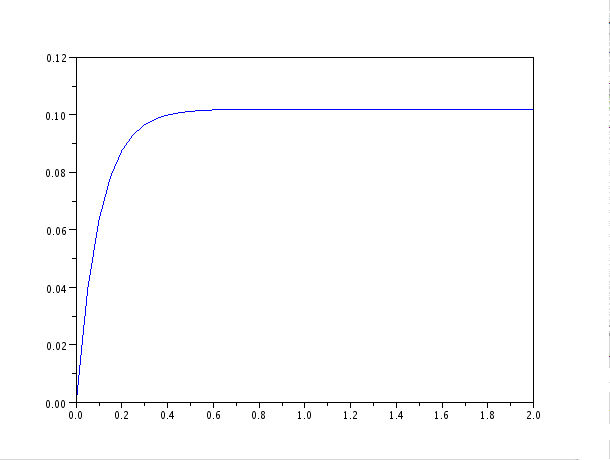
\includegraphics[width=\textwidth]{img/ej01.png}
\caption{Volumen del sistema 1.4 a lo largo de 2s}
\label{fig:p1.1}
\end{figure}

  \item[P1.2] Solucion libre de un sistema de segundo orden
        Para el sistema (1.5):
        \begin{enumerate}[a)]
        \item Reescribir la ecuación de forma matricial
        \item Calcular y graficar la solución con condiciones iniciales $c_{e}(0)=1$, $c_{s}(0)=0$, considerando los parámetros $r_{a}=2$ y $r_{e}=1$
        \item Repetir el punto anterior los parámetros $r_{a}=20$, $r_{e}=1$ y para $r_{a} = 0.1$, $r_{e}=1$.
        \end{enumerate}

        \begin{enumerate}[a)]
\item
\begin{equation}
\left\{ \begin{array}{rl}
  \dot{c_{e}}(t) &= -r_{a} \cdot c_{e}(t) \\
  \dot{c_{s}}(t) &= r_{a} \cdot c_{e}(t) - r_{e} \cdot c_{s}(t)
       \end{array} \right .
 \label{P1.1a} \tag{1.5}
\end{equation}

\begin{equation*}
\begin{bmatrix}
   \dot{c_{e}}(t) \\
   \dot{c_{s}}(t) 
 \end{bmatrix}
=
\begin{bmatrix}
   - r_{a} & 0 \\
     r_{a} & -r_{e}
\end{bmatrix} 
\cdot 
\begin{bmatrix}
   c_{e}(t) \\
   c_{s}(t) 
\end{bmatrix}
\end{equation*}

\item
\begin{figure}[H]
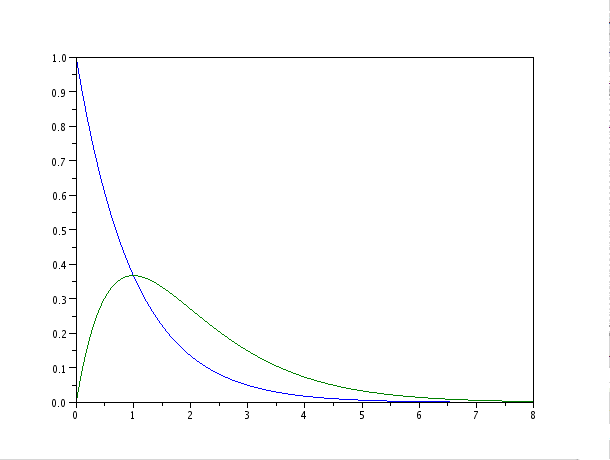
\includegraphics[width=\textwidth]{img/ej02-b.png}
\caption{$c_{e}(0)=1$, $c_{s}(0)=0$, $r_{a}=2$ y $r_{e}=1$ }
\end{figure}

\item
\begin{figure}[H]
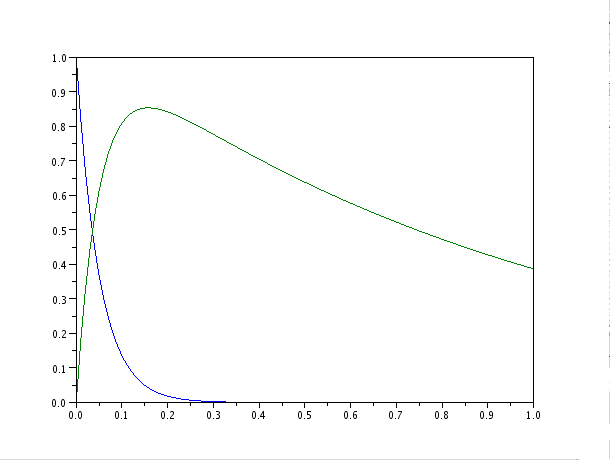
\includegraphics[width=\textwidth]{img/ej02-c1.png}
\caption{$c_{e}(0)=1$, $c_{s}(0)=0$, $r_{a}=20$ y $r_{e}=1$ }
\end{figure}

\begin{figure}[H]
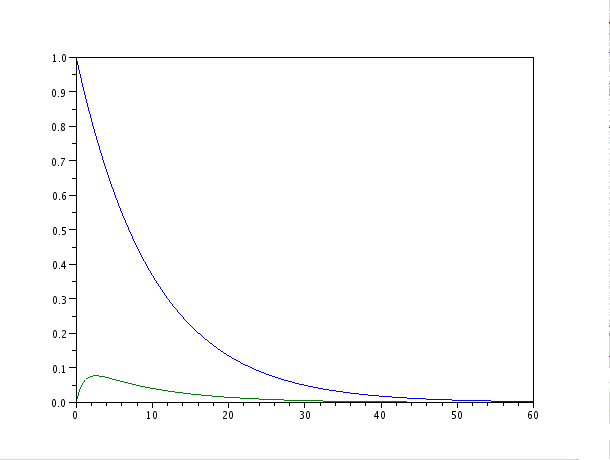
\includegraphics[width=\textwidth]{img/ej02-c2.png}
\caption{$c_{e}(0)=1$, $c_{s}(0)=0$, $r_{a}=0.1$ y $r_{e}=1$ }
\end{figure}

\end{enumerate}

  \item[P1.3] Respuesta al escalón de un sistema de segundo orden para el sistema masa resorte (1.7):
        \begin{enumerate}[a)]
        \item Reescribir la ecuación en forma matricial.
        \item Calcular y graficar la solución considerando condiciones iniciales nulas y que la fuerza de entrada es un escalón unitario, $F(t)=\epsilon(t)$ definido en la Ec(P1.1a). Suponer que los parámetros valen $m=k=b=1$.
        \end{enumerate}

\begin{enumerate}[a)]
        \item
\begin{equation}
\left\{ \begin{array}{rl}
  \dot{x}(t) &= v(t) \\
  \dot{v}(t) &= - \frac{k}{m} \cdot x(t) - \frac{b}{m} \cdot v(t) + \frac{1}{m} \cdot F(t)
       \end{array} \right .
 \label{P1.1a} \tag{1.5}
\end{equation}

\begin{equation*}
\begin{bmatrix}
   \dot{x}(t) \\
   \dot{v}(t) 
 \end{bmatrix}
=
\begin{bmatrix}
   1 & 0 \\
  - \frac{k}{m} &  - \frac{b}{m}
\end{bmatrix} 
\cdot 
\begin{bmatrix}
   x(t) \\
   v(t) 
\end{bmatrix}
+
\begin{bmatrix}
   0 \\
\frac{1}{m}
\end{bmatrix}
\cdot
F(t)
\end{equation*}

\begin{figure}[H]
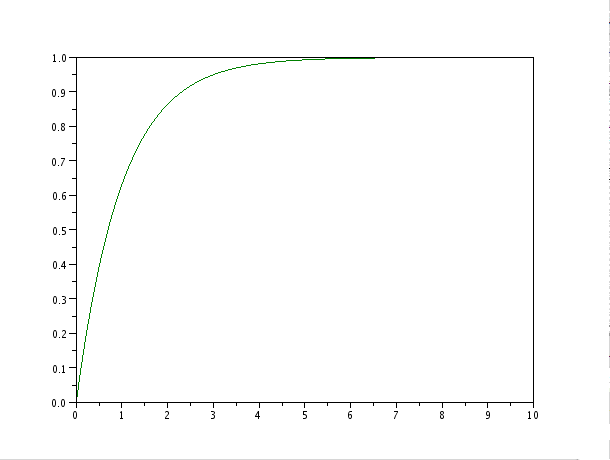
\includegraphics[width=\textwidth]{img/ej03b.png}
\caption{}
\end{figure}



\end{enumerate}
  \item[P1.4] Transformación de una DAE en una ODE explícita. Convertir la DAE (1.9)-(1.10) en una ecuación diferencial ordinaria y escribirla en forma matricial.

\begin{equation*}
\left\{ \begin{array}{rl}
  \dot{u_{c}}(t) &= \frac{1}{C} \cdot i_{L}(t) + \frac{1}{R_{2} \cdot C} u_{L}(t)\\
  \dot{i_{L}}(t) &= - \frac{1}{L} \cdot u_{L}(t) \\
  U(t) &= R_{1} \cdot i_{L}(t) - u_{C}(t) - (1+ \frac{R_{1}}{R_{2}}) \cdot u_{L}(t)
       \end{array} \right .
\end{equation*}

\begin{equation*}
\left\{ \begin{array}{rl}
  \dot{u_{c}}(t) &= (\frac{1}{C} - \frac{R_{1}}{C\cdot (R_{1} + R_{2})}) \cdot i_{L}(t) - \frac{1}{C \dot (R_{1} + R_{2})} \cdot u_{L}(t) + \frac{1}{C \cdot (R_1 + R_2)} \cdot U(t)\\
  \dot{i_{L}}(t) &= - \frac{R_1 \cdot R_2}{L \cdot (R_1 + R_2)} \cdot i_L(t) - \frac{R_1}{L\cdot (R_1 + R_2)} \cdot u_C(t) + \frac{R_2}{L \cdot (R_1+R_2)} \cdot U(t)
       \end{array} \right .
\end{equation*}

\begin{equation*}
\begin{bmatrix}
   \dot{i_C}(t) \\
   \dot{u_L}(t) 
 \end{bmatrix}
=
\begin{bmatrix}
  - \frac{R_1 \cdot R_2}{L\cdot (R_1+R_2)} &  \frac{R_2}{L\cdot (R_1 + R_2)} \\
  \frac{1}{C} \cdot (1 - \frac{R_1}{(R_1+R_2)} & - \frac{1}{C \cdot (R_1 + R_2)} 
\end{bmatrix} 
\cdot 
\begin{bmatrix}
   i_C(t) \\
   u_L(t) 
\end{bmatrix}
+
\begin{bmatrix}
   \frac{R_2}{L\cdot(R_1+R_2)} \\
   \frac{1}{C \cdot (R_1+R_2)}
\end{bmatrix}
\cdot
U(t)
\end{equation*}





  \item[P1.5] Estabilidad de los sitemas lineales y estacionarios. Analizar la estabilidad de los sistemas de los Ejemplos 1.1, 1.3, 1.4, 1.5 y 1.7. Considerar en todos los casos que todos los parametros son positivos.

  \item[P1.6] Punto de equilibrio de un sistema lineal y estacionario. Para el sistema hidráulico (1.4), considerando $Q(t)=\bar{Q}$ (constante) y los parámetros utilizandos en el Problema P1.1, calcular el \textit{punto de equilibrio}. Es decir, se pide cualcular el valor del estado (en este caso $V(t)$) para el cual la solución queda en un estado estacionario ($\dot{V}(t)=0$)
Corroborar luego este resultado con la solución del sistema calculada en el Problema P1.1.

   \item[P1.7] Punto de equilibrio en sistemas no lineales Calcular el/los puntos/s de equilibrio de los sistemas:
        \begin{enumerate}[a)]
        \item El sistema (1.3), considerando $b=m=1$, $g=9.8$
        \item El sistema presa-depredador (1.8), suponiendo $r=a=b=m=0.1$. 
        \end{enumerate}

Interpretar los resultados.




   \item[P1.8] Pelota rebotando. El siguiente modelo puede verse como una combinación del sistema (1.3) (suponiendo rozamiento lineal y con $v(t)$ positiva hacia arriba) y el sistema (1.7) (con $F(t)=-m.g$):

\begin{align*}
  \dot{x}(t) &= v(t) \\
 \label{P1.8a} \tag{P1.8a}
  \dot{v}(t) &=   \begin{cases}
    -\frac{b_{a}}{m} \cdot v(t) - g & \text{si } x(t) > 0\\
    -\frac{k}{m} \cdot x(t) - \frac{b}{m} \cdot v(t) - g & \text {si} x \leq 0,
  \end{cases}\\
\end{align*}
\end{itemize}

Este sistam puede representar un modelo simplificado de una pelota que rebota contra el piso. Cuando $x(t) > 0$ la pelota está en el aire y cuando $x(t) \leq 0$ la pelota está en contacto con el piso y se modeliza como un sistema "masa resorte"

Desde el punto de vista matemático, la ecuación (7.1) es seccionalmente lineal ó lineal a tramos. Si bien no se puede calcular la solución analítica en forma exacta, es posible calcular tramos de la solución.

Considerando entonces los parámetros $b_{a} = 0.1$, $m=1$, $b=30$, $g=9.8$ y $k = 100000$, se pide:
\begin{enumerate}[a)]
\item Calcular y graficar un tramo de la solución desde la condición inicial $x(0)=10$, $v(0)=0$, hasta el tiempo $t_{1}$, en el que se verifique $x(t_{1})=0$.
Ayuda: Como la matriz $A$ es singular es este caso no puede calcularse la integral de $e^{A \cdot t}$ como $A^{-1} \cdot e^{A \cdot t}$. Una opción (para seguir utilizando esta forma de integrar) es modificar la matriz $A$, agregando un pequeño término que evite que sea singular.

Además notar que para calcular el tiempo $t_{1}$ va a ser necesario utilizar alguna forma de iteración.

\item Utiliando como condición inicial los valores finales del tramo obtenido en el punto anterior: $x(t_{1})(=0)$, $v(t_{1})$, calcular un nuevo tramo de la solución hasta un instante $t_{2}$ en que se verifique nuevamente $x(t_{2})=0$.

\item Repetir el punto anterior varias veces y graficar la solución obtenida.
\end{enumerate}

\end{document}
